\documentclass[tikz,border=10pt]{standalone}
\usepackage[T1]{fontenc}
\usepackage{lmodern}
\usepackage{tikz}
\usetikzlibrary{arrows.meta,calc,decorations.pathreplacing,fit,matrix,positioning}

\definecolor{cornellred}{HTML}{B31B1B}
\definecolor{ink}{HTML}{202124}
\definecolor{muted}{HTML}{667085}
\definecolor{line}{HTML}{AEB8C6}
\definecolor{paper}{HTML}{FFFFFF}
\definecolor{soft}{HTML}{F5F7FA}
\definecolor{camera}{HTML}{E8F4FF}
\definecolor{memory}{HTML}{F0F7EC}
\definecolor{compute}{HTML}{FFF3E6}
\definecolor{display}{HTML}{F7ECF3}
\definecolor{verify}{HTML}{EFEAFE}

\tikzset{
  font=\sffamily,
  flow/.style={
    -{Latex[length=2.6mm,width=1.8mm]},
    draw=muted,
    line width=0.8pt,
    rounded corners=2pt
  },
  dataflow/.style={
    flow,
    draw=cornellred
  },
  block/.style={
    rectangle,
    rounded corners=3pt,
    draw=line,
    line width=0.8pt,
    fill=paper,
    align=center,
    minimum width=28mm,
    minimum height=10mm,
    inner xsep=4pt,
    inner ysep=4pt
  },
  smallblock/.style={
    block,
    minimum width=22mm,
    minimum height=8mm,
    font=\sffamily\scriptsize
  },
  title/.style={
    font=\sffamily\bfseries\large,
    text=ink
  },
  labeltext/.style={
    font=\sffamily\scriptsize,
    text=muted,
    align=center
  },
  camera_block/.style={block, fill=camera, draw=blue!45!black},
  memory_block/.style={block, fill=memory, draw=green!45!black},
  compute_block/.style={block, fill=compute, draw=orange!65!black},
  display_block/.style={block, fill=display, draw=purple!45!black},
  verify_block/.style={block, fill=verify, draw=violet!50!black},
  groupbox/.style={
    draw=line,
    rounded corners=5pt,
    line width=0.7pt,
    fill=soft,
    inner sep=7pt
  }
}

\usetikzlibrary{arrows.meta,positioning,fit,calc,decorations.pathreplacing}

\begin{document}
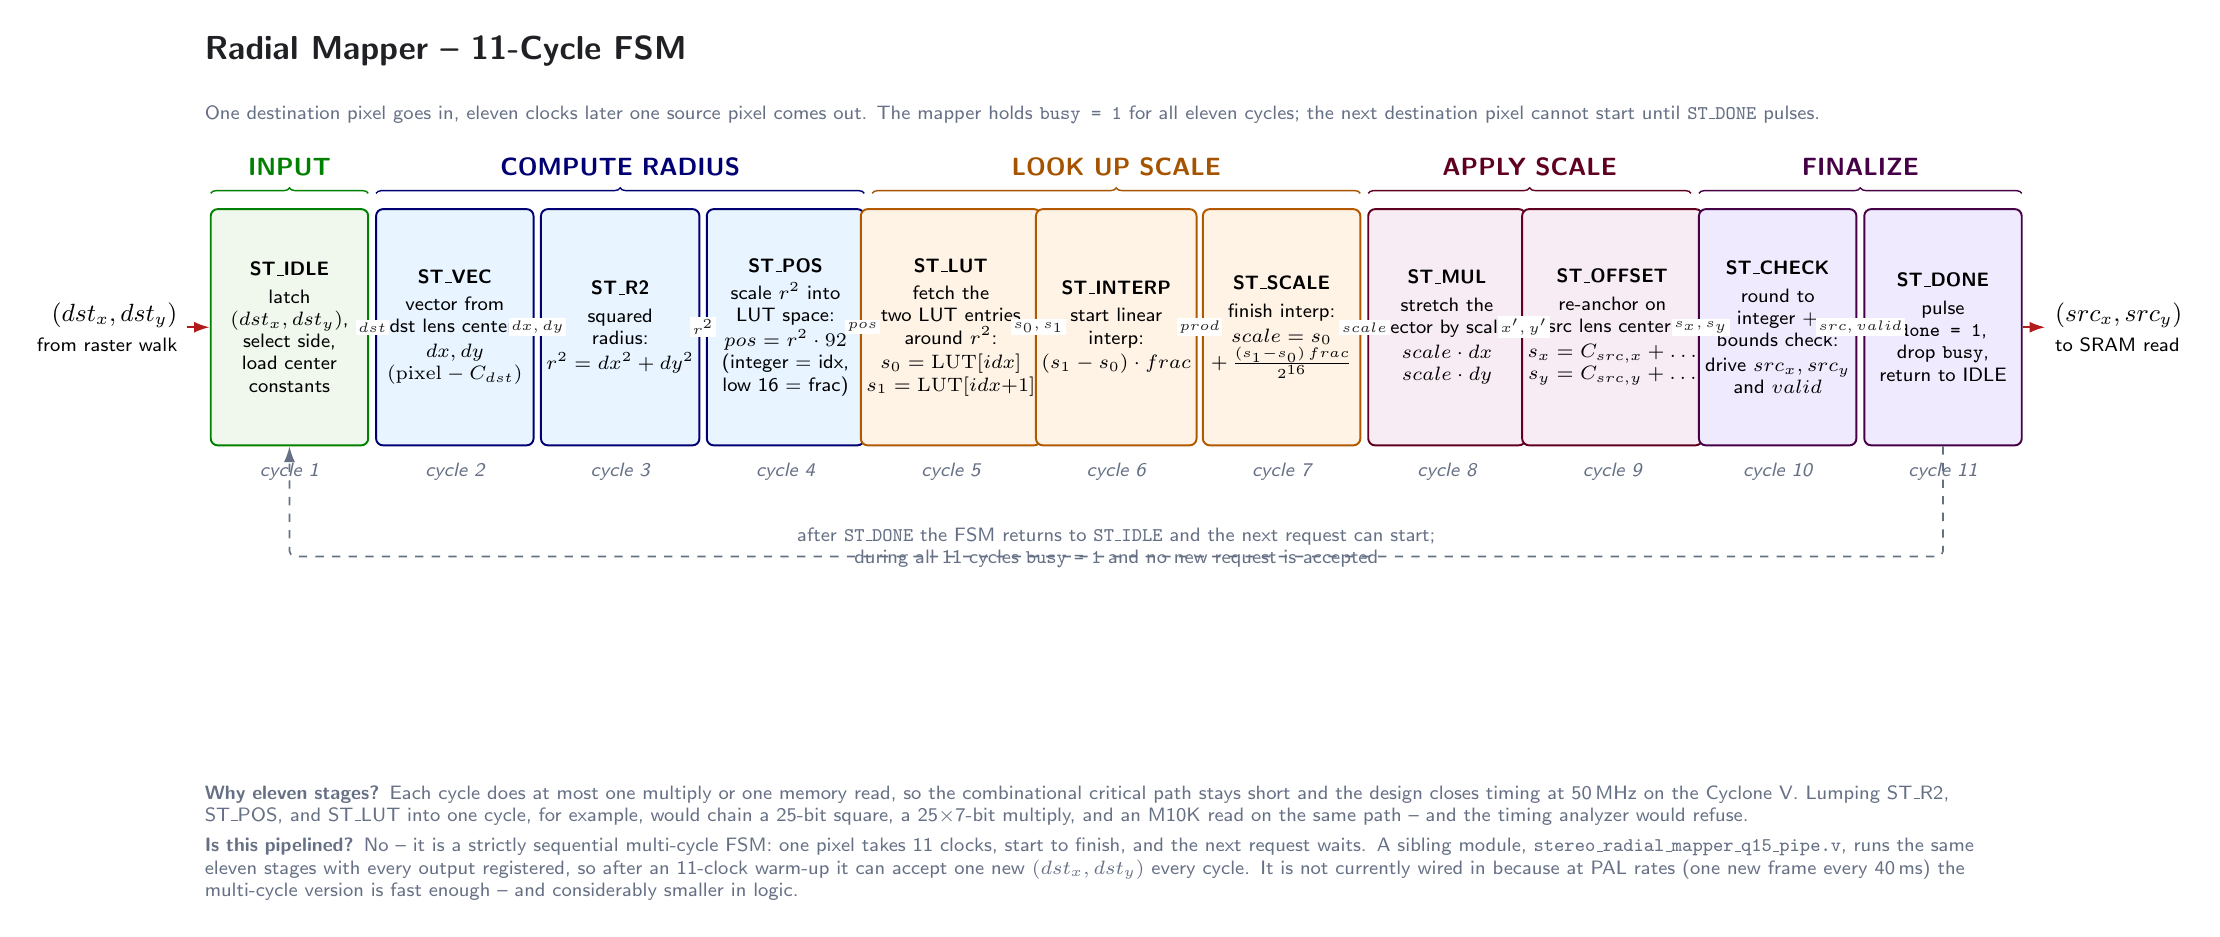
\begin{tikzpicture}[x=1mm,y=1mm,
  st/.style={
    rectangle, rounded corners=2.5pt,
    draw=line, line width=0.7pt,
    fill=paper, align=center,
    font=\sffamily\scriptsize,
    minimum width=20mm, minimum height=30mm,
    inner xsep=2pt, inner ysep=2pt
  },
  st_in/.style    ={st, fill=memory,  draw=green!50!black},
  st_radius/.style={st, fill=camera,  draw=blue!45!black},
  st_lut/.style   ={st, fill=compute, draw=orange!70!black},
  st_apply/.style ={st, fill=display, draw=purple!50!black},
  st_out/.style   ={st, fill=verify,  draw=violet!55!black},
  pipe/.style={
    -{Latex[length=2.0mm,width=1.4mm]},
    draw=cornellred, line width=0.8pt
  },
  cyc/.style={font=\sffamily\scriptsize\itshape, text=muted},
  flowlbl/.style={font=\sffamily\tiny, text=ink,
    fill=paper, inner sep=1pt}
]

  \node[title, anchor=west] at (0, 130)
    {Radial Mapper -- 11-Cycle FSM};
  \node[labeltext, anchor=west, align=left] at (0, 122)
    {One destination pixel goes in, eleven clocks later one source pixel comes out.
     The mapper holds \texttt{busy = 1} for all eleven cycles; the next destination
     pixel cannot start until \texttt{ST\_DONE} pulses.};

  %====================================================================
  % Phase header brackets (above the boxes)
  %====================================================================
  \node[labeltext, anchor=south, font=\sffamily\small\bfseries,
        text=green!50!black] at (12, 113) {INPUT};
  \draw[decorate, decoration={brace, amplitude=2pt, raise=0pt},
        draw=green!50!black, line width=0.5pt] (2, 112) -- (22, 112);

  \node[labeltext, anchor=south, font=\sffamily\small\bfseries,
        text=blue!45!black] at (54, 113) {COMPUTE RADIUS};
  \draw[decorate, decoration={brace, amplitude=2pt, raise=0pt},
        draw=blue!45!black, line width=0.5pt] (23, 112) -- (85, 112);

  \node[labeltext, anchor=south, font=\sffamily\small\bfseries,
        text=orange!65!black] at (117, 113) {LOOK UP SCALE};
  \draw[decorate, decoration={brace, amplitude=2pt, raise=0pt},
        draw=orange!65!black, line width=0.5pt] (86, 112) -- (148, 112);

  \node[labeltext, anchor=south, font=\sffamily\small\bfseries,
        text=purple!50!black] at (169.5, 113) {APPLY SCALE};
  \draw[decorate, decoration={brace, amplitude=2pt, raise=0pt},
        draw=purple!50!black, line width=0.5pt] (149, 112) -- (190, 112);

  \node[labeltext, anchor=south, font=\sffamily\small\bfseries,
        text=violet!55!black] at (211.5, 113) {FINALIZE};
  \draw[decorate, decoration={brace, amplitude=2pt, raise=0pt},
        draw=violet!55!black, line width=0.5pt] (191, 112) -- (232, 112);

  %====================================================================
  % The 11 state boxes
  %====================================================================
  % cycle 1
  \node[st_in]     (s1)  at ( 12, 95)
    {\textbf{ST\_IDLE}\\[2pt]
     latch\\$(dst_x, dst_y)$,\\select side,\\load center\\constants};

  % cycle 2
  \node[st_radius] (s2)  at ( 33, 95)
    {\textbf{ST\_VEC}\\[2pt]
     vector from\\dst lens center:\\[1pt]
     $dx, dy$\\\scriptsize{}$(\mathrm{pixel} - C_{dst})$};

  % cycle 3
  \node[st_radius] (s3)  at ( 54, 95)
    {\textbf{ST\_R2}\\[2pt]
     squared\\radius:\\[1pt]
     $r^2 = dx^2 + dy^2$};

  % cycle 4
  \node[st_radius] (s4)  at ( 75, 95)
    {\textbf{ST\_POS}\\[2pt]
     scale $r^2$ into\\LUT space:\\[1pt]
     $pos = r^2 \cdot 92$\\\scriptsize{}(integer = idx,\\\scriptsize{}low 16 = frac)};

  % cycle 5
  \node[st_lut]    (s5)  at ( 96, 95)
    {\textbf{ST\_LUT}\\[2pt]
     fetch the\\two LUT entries\\around $r^2$:\\[1pt]
     $s_0 = \mathrm{LUT}[idx]$\\$s_1 = \mathrm{LUT}[idx{+}1]$};

  % cycle 6
  \node[st_lut]    (s6)  at (117, 95)
    {\textbf{ST\_INTERP}\\[2pt]
     start linear\\interp:\\[1pt]
     $(s_1 - s_0)\cdot frac$};

  % cycle 7
  \node[st_lut]    (s7)  at (138, 95)
    {\textbf{ST\_SCALE}\\[2pt]
     finish interp:\\[1pt]
     $scale = s_0$\\$+\,\frac{(s_1{-}s_0)\,frac}{2^{16}}$};

  % cycle 8
  \node[st_apply]  (s8)  at (159, 95)
    {\textbf{ST\_MUL}\\[2pt]
     stretch the\\vector by scale:\\[1pt]
     $scale \cdot dx$\\$scale \cdot dy$};

  % cycle 9
  \node[st_apply]  (s9)  at (180, 95)
    {\textbf{ST\_OFFSET}\\[2pt]
     re-anchor on\\src lens center:\\[1pt]
     $s_x = C_{src,x} + \ldots$\\$s_y = C_{src,y} + \ldots$};

  % cycle 10
  \node[st_out]    (s10) at (201, 95)
    {\textbf{ST\_CHECK}\\[2pt]
     round to\\integer +\\bounds check:\\[1pt]
     drive $src_x, src_y$\\and $valid$};

  % cycle 11
  \node[st_out]    (s11) at (222, 95)
    {\textbf{ST\_DONE}\\[2pt]
     pulse\\\texttt{done = 1},\\drop \texttt{busy},\\return to IDLE};

  %====================================================================
  % Cycle labels below each box
  %====================================================================
  \foreach \i/\xc in {1/12, 2/33, 3/54, 4/75, 5/96, 6/117, 7/138, 8/159, 9/180, 10/201, 11/222} {
    \node[cyc, anchor=north] at (\xc, 79) {cycle \i};
  }

  %====================================================================
  % Inter-state arrows with the registered value carried between cycles
  %====================================================================
  \draw[pipe] (s1.east)  -- node[flowlbl]{$dst$} (s2.west);
  \draw[pipe] (s2.east)  -- node[flowlbl]{$dx,dy$} (s3.west);
  \draw[pipe] (s3.east)  -- node[flowlbl]{$r^2$} (s4.west);
  \draw[pipe] (s4.east)  -- node[flowlbl]{$pos$} (s5.west);
  \draw[pipe] (s5.east)  -- node[flowlbl]{$s_0,s_1$} (s6.west);
  \draw[pipe] (s6.east)  -- node[flowlbl]{$prod$} (s7.west);
  \draw[pipe] (s7.east)  -- node[flowlbl]{$scale$} (s8.west);
  \draw[pipe] (s8.east)  -- node[flowlbl]{$x',y'$} (s9.west);
  \draw[pipe] (s9.east)  -- node[flowlbl]{$s_x,s_y$} (s10.west);
  \draw[pipe] (s10.east) -- node[flowlbl]{$src,valid$} (s11.west);

  %====================================================================
  % Input / output anchors
  %====================================================================
  \node[font=\sffamily\small, anchor=east, align=right] (input) at (-1, 95)
    {$(dst_x, dst_y)$\\\scriptsize{}from raster walk};
  \draw[pipe] (input.east) -- (s1.west);

  \node[font=\sffamily\small, anchor=west, align=left] (output) at (235, 95)
    {$(src_x, src_y)$\\\scriptsize{}to SRAM read};
  \draw[pipe] (s11.east) -- (output.west);

  %====================================================================
  % "Not pipelined" feedback loop, drawn under the boxes
  %====================================================================
  \draw[pipe, draw=muted, dashed, line width=0.6pt,
        rounded corners=2pt]
    (s11.south) -- ++(0,-14) -| (s1.south);
  \node[font=\sffamily\scriptsize, text=muted, align=center,
        text width=120mm] at (117, 67)
    {after \texttt{ST\_DONE} the FSM returns to \texttt{ST\_IDLE} and the next request can start;\\
     during all 11 cycles \texttt{busy = 1} and no new request is accepted};

  %====================================================================
  % Footer
  %====================================================================
  \node[labeltext, anchor=north west, align=left, text width=230mm] at (0, 38)
    {\textbf{Why eleven stages?} Each cycle does at most one multiply or one memory read, so the combinational critical path stays short and the design closes timing at 50\,MHz on the Cyclone V. Lumping ST\_R2, ST\_POS, and ST\_LUT into one cycle, for example, would chain a 25-bit square, a 25$\times$7-bit multiply, and an M10K read on the same path -- and the timing analyzer would refuse.\\[3pt]
     \textbf{Is this pipelined?} No -- it is a strictly sequential multi-cycle FSM: one pixel takes 11 clocks, start to finish, and the next request waits. A sibling module, \texttt{stereo\_radial\_mapper\_q15\_pipe.v}, runs the same eleven stages with every output registered, so after an 11-clock warm-up it can accept one new $(dst_x, dst_y)$ every cycle. It is not currently wired in because at PAL rates (one new frame every 40\,ms) the multi-cycle version is fast enough -- and considerably smaller in logic.};

\end{tikzpicture}
\end{document}
